\documentclass[submit]{harvardml}

% Put in your full name and email address.
\name{Aditya N. Prasad}
\email{\small adityaprasad@college.harvard.edu}

% List any people you worked with.
\collaborators{%
  None
}

% You don't need to change these.
\course{CS281-F17}
\assignment{Assignment \#1 v 1.0}
\duedate{11:59pm September 22, 2017}

\usepackage{url, enumitem}
\usepackage{amsfonts}
\usepackage{listings}
\usepackage{bm}
\usepackage{todonotes}
\usepackage{booktabs}
% Some useful macros.
\newcommand{\given}{\,|\,}
\newcommand{\R}{\mathbb{R}}
\newcommand{\E}{\mathbb{E}}
\newcommand{\var}{\text{var}}
\newcommand{\cov}{\text{cov}}
\newcommand{\N}{\mathcal{N}}
\newcommand{\ep}{\varepsilon}

\newcommand{\Dir}{\text{Dirichlet}}
\newcommand{\D}{\text{Dir}}
\newcommand{\Cat}{\text{Cat}}
\renewcommand{\v}{\boldsymbol}

\DeclareMathOperator*{\argmax}{arg\,max}

\newtheorem*{theorem}{Theorem}
\begin{document}

%%%%%%%%%%%%%%%%%%%%%%%%%%%%%%%%%%%%%%%%%%%%%%%%%%%%%%%%
%%%%%%%%%%%%%%%%% PROBLEM 1 %%%%%%%%%%%%%%%%%%%%%%%%%%%%
%%%%%%%%%%%%%%%%%%%%%%%%%%%%%%%%%%%%%%%%%%%%%%%%%%%%%%%%
\begin{problem}[A Classic on the Gaussian Algebra, 10pts]
  Let $X$ and $Y$ be independent univariate Gaussian random
 variables. In the previous problem set, you likely used the closure property that $Z = X + Y$ is also a Gaussian random variable. Here you'll prove this fact.
\begin{enumerate}[label=(\alph*)]
\item Suppose $X$ and $Y$ have mean 0 and variances $\sigma_X^2$ and $\sigma_Y^2$ respectively. Write the pdf of $X + Y$ as an integral.
\item Evaluate the integral from the previous part to find a closed-form expression for the pdf of $X+Y$, then argue that this expression implies that $X+Y$ is also Gaussian with mean $0$ and variance $\sigma_X^2 + \sigma_Y^2$. Hint: what is the integral, over the entire real line, of
\[
f(x) = \frac{1}{\sqrt{2\pi}\sigma} \exp\left( -\frac{1}{2\sigma^2}(x - \mu)^2 \right) ,
\] i.e., the pdf of a univariate Gaussian random variable?
\item Extend the above result to the case in which $X$ and $Y$ may have arbitrary means.
\item Univariate Gaussians are supported on the entire real line. Sometimes this is undesirable because we are modeling a quantity with positive support. A common way to transform a Gaussian to solve this problem is to exponentiate it. Suppose $X$ is a univariate Gaussian with mean $\mu$ and variance $\sigma^2$. What is the pdf of $e^X$?
\end{enumerate}
\vspace{0.1cm}
\end{problem}

\begin{enumerate}[label=(\alph*)]
	\item We write a simple proof that the probability sum of independent rvs corresponds to their convolution for discrete variables. This corresponds directly to the continuous case with PMFs replaced by PDFs and sums replaced by integrals. Let $X$ and $Y$ be independent random variables and $Z = X+Y$. Then,
		\begin{align*}
			P(Z = k) &= P(X + Y = k) \\
					&= \sum_{x} P(X + Y = k, X= x) \\
					&= \sum_{x}P(Y=k -x \given X = x) P(X = x)\\
					&= \sum_{x}P(Y= k-x) P(X=x)
		\end{align*}
	
	In our case, we have: $X \sim \N(0, \sigma_{x}^2)$ and $Y \sim \N(0, \sigma_{y}^2)$. The pdf of the sum, denoted $Z$, is simply the convolution:
		\begin{align*}
			f_{Z}(z) &= f_{X+Y}(z) \\
					&= \int_{-\infty}^{\infty} f_{Y|X} (z-x | x) f_{X}(x) dx \\
					&= \int_{-\infty}^{\infty} f_{Y} (z-x)f_{X}(x) dx \\
					&= \left(\frac{1}{\sigma_x\sqrt{2\pi}} \right)\left(\frac{1}{\sigma_y\sqrt{2\pi}} \right) \int_{-\infty}^{\infty} e^{-\frac{1}{2\sigma_x^2}x^2} e^{-\frac{1}{2\sigma_y^2}(z-x)^2} dx
		\end{align*}
	\item To evaluate this integral neatly, we complete separate the dependence on $z$ and $x$, whilst completing the square on $x$ so that its integral is Gaussian in form. Consider the negative of the exponent:
		\begin{align*}
			\frac{x^2}{2\sigma_x^2} + \frac{(x-z)^2}{2\sigma_y^2} &= \frac{x^2\sigma_y^2 + (x-z)^2\sigma_x^2}{2\sigma_x^2\sigma_y^2}\\
&= \frac{x^2(\sigma_x^2 + \sigma_y^2)}{2\sigma_x^2\sigma_y^2} + \frac{(z^2-2zx)(\sigma_x^2 + \sigma_y^2)\sigma_x^2}{2\sigma_x^2\sigma_y^2(\sigma_x^2 + \sigma_y^2)} \\
&= \frac{\left(\frac{z^2\sigma_x^4}{\sigma_x^2 + \sigma_y^2} \right) - x\left(2z\sigma_x^2 \right) + x^2(\sigma_x^2 + \sigma_y^2)}{2\sigma_x^2\sigma_y^2}  + \frac{z^2}{2(\sigma_x^2 + \sigma_y^2)} \\
&=  \frac{\left[x - \left(\frac{z\sigma_x^2}{\sigma_x^2 + \sigma_y^2} \right)\right]^2}{2\left(\frac{\sigma_x^2\sigma_y^2}{\sigma_x^2 + \sigma_y^2} \right)} +      \frac{z^2}{2(\sigma_x^2 + \sigma_y^2)}   \\
&= \frac{1}{2} \left(\frac{x - \mu^2}{\sigma^{'}}\right)^2 +  \frac{z^2}{2(\sigma_x^2 + \sigma_y^2)}
		\end{align*}
		
		Therefore, we have:
		\begin{align*}
			f_{Z}(z) &= \left(\frac{1}{\sigma_x\sqrt{2\pi}} \right)\left(\frac{1}{\sigma_y\sqrt{2\pi}} \right) \int_{-\infty}^{\infty} \exp\left({-\frac{1}{2\sigma_x^2}x^2} + -\frac{1}{2\sigma_y^2}(z-x)^2 \right) dx \\
					&= \left(\frac{1}{\sigma_x\sqrt{2\pi}} \right)\left(\frac{1}{\sigma_y\sqrt{2\pi}} \right) \int_{-\infty}^{\infty} \exp{\left( -\frac{1}{2}\left(\frac{x - \mu^2}{\sigma^{'}}\right)^2 - \frac{z^2}{2(\sigma_x^2 + \sigma_y^2)} \right)} dx \\
					&= \left( -\frac{1}{\sigma_x \sigma_y 2\pi} \right) \exp{\left(-\frac{z^2}{2(\sigma_x^2 + \sigma_y^2)} \right)}\int_{-\infty}^{\infty}\exp{\frac{1}{2}\left(\frac{x - \mu^2}{\sigma^{'}}\right)^2}dx \\
					&= \left( \frac{1}{\sigma_x \sigma_y 2\pi} \right) \exp{\left(\frac{-z^2}{2(\sigma_x^2 + \sigma_y^2)} \right)} \sqrt{2\pi} \sigma' \\
					&= \frac{1}{\sqrt{2\pi(\sigma_x^2 + \sigma_y^2)}}\exp{\left(-\frac{z^2}{2(\sigma_x^2 + \sigma_y^2)}\right)}
		\end{align*}
		
		Therefore, $Z \sim \N(0, \sigma^2_x + \sigma^2_y)$.
	
	\item This is simply corresponds to a translation of the random-variable. More concretely, assume $X' \sim \N(\mu_x, \sigma_x^2)$ and $Y' \sim \N(\mu_y, \sigma_y^2)$. Then, $Z' = X' + Y'$ is :
		\begin{align*}
			Z' &=  X' + Y' \\
			   &= (X + \mu_x) + (Y + \mu_y) \tag{where $X \sim \N(0, \sigma_{x}^2), Y \sim \N(0, \sigma_{y}^2)$} \\
			   &= (X+Y) + (\mu_x + \mu_y) \\
			   &= Z + \mu'
		\end{align*}
		Therefore, $Z \sim \mathcal{N}(\mu_x + \mu_y, \sigma_x^2 + \sigma_y^2)$.
	\item We write this in terms of CDFs. Let $Y = \exp(X)$. We note that the exponential function is monotonic, and that $y \in [0, \infty$. 
		\begin{align*}
			F_Y(y) = P(Y \leq y) = P(g(X) \leq y) = P(X \leq \log y) = \Phi(\log y)
		\end{align*}
		Here, $\Phi$ is the CDF of the univariate normal. The PDF is therefore:
		\begin{align*}
			f_Y(y) = \partial{y} F_Y(y) = \psi(\log y)\frac{1}{y}, \space y >0
		\end{align*}
\end{enumerate}
\pagebreak
%%%%%%%%%%%%%%%%%%%%%%%%%%%%%%%%%%%%%%%%%%%%%%%%%%%%%%%%
%%%%%%%%%%%%%%%%% PROBLEM 2 %%%%%%%%%%%%%%%%%%%%%%%%%%%%
%%%%%%%%%%%%%%%%%%%%%%%%%%%%%%%%%%%%%%%%%%%%%%%%%%%%%%%%
\begin{problem}[Regression, 13pts]
Suppose that $X \in \R^{n \times m}$ with $n \geq m$ and $Y \in \R^n$, and that $Y \sim \N(Xw, \sigma^2 I)$. You learned in class that the maximum likelihood estimate $\hat{w}$ of ${w}$ is given by
\[
\hat{w} = (X^TX)^{-1}X^TY
\]
\begin{enumerate}[label=(\alph*)]
\item Why do we need to assume that $n \geq m$?
\item Define $H = X(X^TX)^{-1}X^T$, so that the ``fitted" values $\hat Y = X\hat{{w}}$ satisfy $\hat Y = HY$. Show that $H$ is an orthogonal projection matrix that projects onto the column space of $X$, so that the fitted y-values are a projection of $Y$ onto the column space of $X$.
\item What are the expectation and covariance matrix of $\hat{w}$?
\item Compute the gradient with respect to ${w}$ of the log likelihood implied by the model above, assuming we have observed $Y$ and $X$.
\item Suppose we place a normal prior on ${w}$. That is, we assume that ${w} \sim \N(0, \tau^2 I)$. Show that the MAP estimate of ${w}$ given $Y$ in this context is
\[
\hat {w}_{MAP} = (X^TX + \lambda I)^{-1}X^T Y
\]
where $\lambda = \sigma^2 / \tau^2$. (You may employ standard conjugacy results about Gaussians without proof in your solution.)

[Estimating ${w}$ in this way is called {\em ridge regression} because the matrix $\lambda I$ looks like a ``ridge''. Ridge regression is a common form of {\em regularization} that is used to avoid the overfitting (resp. underdetermination) that happens when the sample size is close to (resp. higher than) the output dimension in linear regression.]
\item Do we need $n \geq m$ to do ridge regression? Why or why not?
\item Show that ridge regression is equivalent to adding $m$ additional rows to $X$ where the $j$-th additional row has its $j$-th entry equal to $\sqrt{\lambda}$ and all other entries equal to zero, adding $m$ corresponding additional entries to $Y$ that are all 0, and then computing the maximum likelihood estimate of ${w}$ using the modified $X$ and $Y$.
\end{enumerate}
\vspace{0.1cm}
\end{problem}
For ease of notation, matrices are denoted with boldface uppercase letters, and vectors are denoted with boldface lowercase letters.
\begin{enumerate}[label=(\alph*)]
	\item We first make a purely mathematical argument, and then attempt to provide a reasonable interpretation. Consider the matrix: $\v{X} \in \mathbb{R}^{m \times n}$. For argument's sake, assume $n < m$. Since the row rank equals column rank, the rank of matrix $\v{X}$, denoted here by $\rho(\v{X})$, is at most $n$. That is, 
	\begin{align*}
		\rho(\v{X}) = r \leq n < m
	\end{align*}
	We also have that $\rho(\v{X}) = \rho(\v{X^T X})$. This follows directly from the fact that the null-space, $\mathcal{N}$, of $\v{A}$ is the same as that of $\v{A^T}$ (we provide a full-proof at the end of the problem). Therefore, we have that:
	\begin{align*}
		\rho(\v{X^T X}) = r \leq n < m  (\equiv \text{no. of columns in } \v{X^T X})
	\end{align*}
	
	As such, $\v{X^T X}$ does not have full-rank in columns. With the regression problem as defined above, we know that the condition that maximizes the likelihood function is:
	\begin{align*}
		\v{X^T X} \v{w} = \v{X^T y}
	\end{align*}
	This can be written as:
	\begin{align*}
		\v{A} \v{w} = \v{b}
	\end{align*}
	However, since $\rho(\v{A}) = \rho(\v{X^T X}) = n < m$, there are an infinite number of solutions. Hence, the problem is ill-posed.
	
	There are many ways to interpret this:
	\begin{enumerate}[label=(\roman*)]
		\item Gelman et al. (pg 377) make the argument that in such a regression problem, we cannot uniquely determine parameters because our columns of explanatory variables are not linearly independent. The data is `collinear', or rather, `co-planar'. The data forms a $n$ dimensional subspace/hyperplane of the $m$ dimensional parameter space. The data thus provides very little information about possible linear combinations of $\v{w}$. 
		\item This is similar to the proof above, but perhaps is easier to understand. $\v{X^T X} \v{w} = \v{X^T} \v{y}$ are the normal form equations for the system $\v{X} \v{w} = \v{y}$. Here, $\v{w} \in \mathbb{R}^m$. Therefore, we have a system of equations that looks like:
			\begin{align*}
				\begin{pmatrix}
					x^{1}_1 w_1 + \cdots + x^{1}_m w_m \\
					\vdots \\
					x^{n}_1 w_1 + \cdots + x^{n}_m w_m
				\end{pmatrix} = \begin{pmatrix}
				y_1 \\ \vdots \\ y_n
				\end{pmatrix}
			\end{align*}
			Therefore, in the best case scenario we have $n$ equations for $m$ unknowns ($\v{w}$), where $n<m$. Therefore, we see that we have an infinite number of solutions.
		\item (Geometric Intuition based on projections) \todo{Geometric argument}
	\end{enumerate}
	
	\item The easiest way to show this is to prove that $H$ is idempotent and symmetric, and then show that $\v{X}^T (\v{y} - \v{\hat{y}}) = 0$. We drop the bold-face for ease of typing here.
	\begin{enumerate}[label=(\roman*)]
		\item Idempotence: 
			\begin{align*}
				H^2 &= (X (X^T X)^{-1}X^T ) (X (X^T X)^{-1}X^T ) \\
					&= X (X^T X)^{-1}(X^T X) (X^T X)^{-1} X^T \\
					&= X (X^T X)^{-1}X^T \\
					&= H
			\end{align*}
		
		\item Symmetry (noting  $X^T X$ is obviously symmetric):
			\begin{align*}
				H^T = (X (X^T X)^{-1}X^T )^T = H
			\end{align*}
			
			Therefore, $H$ is an orthogonal, projection operator.
		\item Orthogonality: consider $v = y - H y$. We show that this vector is perpendicular to the column-space of $X$. 
			\begin{align*}
				X^T ( y - H y) &= X^T y - X^T (X (X^T X)^{-1}X^T ) y \\
								&= X^T y - X^T y = 0
			\end{align*}
			Therefore, all the columns of $X$ are perpendicular to $(y-Hy)$. Therefore, $Hy$ is the projection of $y$ onto the column-space of $X$.
	\end{enumerate}
	
There is a more sophisticated and general way of making the last point. This has been adapted from \textit{Bhattacharya \& Roy, Linear Algebra and Matrix Analysis for Statistics}.
	\begin{theorem}
		If $\v{y} \in \mathbb{R}^n$ and $\v{X} \in \mathbb{R}^{n \times m}$, the orthogonal projection of $y$ onto the column-space of $\v{X}$, denoted $\v{w} \in \mathbb{R}^m$ satisfies the normal equations:
			\begin{align*}
				\v{X^T X w} = \v{X^T y}
			\end{align*}
	\end{theorem}
	The maximum-likelihood estimate of the weights is thus a distribution (because of it's dependence on Y) even though the weights themselves are simply parameters.
	\begin{proof}
		We know that $\mathbb{R}^n$ can be written as the direct sum: $\mathbb{R}^n = \mathcal{C}(X) \oplus \mathcal{C}(X)^{\perp} =  \mathcal{C}(X) \oplus \mathcal{N}(X^T)$. Therefore, we can write $\v{y} \in \mathbb{R}^n$ as:
			\begin{align*}
			y = u + v, \space \left\{u \in \mathcal{C}(X), v  \in \mathcal{N}(X^T) \right \}
			\end{align*}
			Since $u \in \mathcal{C}(X)$, there exists $w \in \mathbb{R}^m$ s.t. $u = X w$. Therefore, we have:
			\begin{align*}
				v = y - u = y - X w
			\end{align*}
			Since $v  \in \mathcal{N}(X^T)$, 
			\begin{align*}
				X^T v = X^T (y - X w) = 0
			\end{align*}
			Therefore,
			\begin{align}
				X^T X w = X^T y
			\end{align}
	\end{proof}
	Further, if $X^T X$ has full-rank, it has an inverse (because it is also square). Therefore, we have:
		\begin{align}
			\v{w} = \v{(X^T X)}^{-1} \v{X^T y}
		\end{align}
	
	\item We are assuming here that $\v{X}$ and $\v{w}$ are parameters. Therefore, we have:
		\begin{align*}
			\E(\v{\hat w}) &= \E(\v{(X^T X)}^{-1} \v{X^T y}) \\
							&= \v{(X^T X)}^{-1} \v{X^T} \E(\v{y}) \\
							&= \v{(X^T X)}^{-1} \v{X^T X} \v{w} \\
							&= \v{w}
		\end{align*}
		
		The covariance matrix is similarly calculated:
		\begin{align}
			\label{eq:cov}
			\cov( \v{\hat w},  \v{\hat w}) &= \E \left[ ( \v{\hat w} - E( \v{\hat w})) ( \v{\hat w} - E( \v{\hat w}))^T\right] \\
			&= \E \left[ \v{\hat w} \v{\hat w}^T \right] - \E \left[\v{\hat w}\right ] \E \left[ \v{\hat w}^T \right]
		\end{align}
		We have:
		\begin{align*}
			\E (\v{\hat w} \v{\hat w}^T) &= \E \left(\v{(X^T X)}^{-1} \v{X^T y} \left [ \v{(X^T X)}^{-1} \v{X^T y} \right]^T \right) \\
			&= \v{(X^T X)}^{-1} \v{X^T} \v{X} \v{(X^T X)}^{-1} \E(\v{y y^T}) \\
			&= \v{(X^T X)}^{-1} \E( \v{y} \v{y^T})
		\end{align*}
		
		Therefore, we have:
		\begin{align}
			\cov( \v{\hat w},  \v{\hat w}) &= \v{(X^T X)}^{-1} \left(\E( \v{y} \v{y^T}) - \E(\v{y}) \E(\v{y}^T) \right) \\
			&= \v{(X^T X)}^{-1} (\sigma^2 \v{I})
		\end{align}
	
	\item We have:
		\begin{align*}
			p(\v{y}; \v{X}, \v{w})  \propto \exp \left[ -\frac{1}{2 \sigma^2} (\v{y} - \v{X} \v{w})^T (\v{y} - \v{X} \v{w}) \right]
		\end{align*}
		Therefore, if we want to maximize the logarithm of this density w.r.t the parameter $\v{w}$, we have:
		\begin{align*}
			\argmax_{\v{w}} \left[ -(\v{y} - \v{X} \v{w})^T (\v{y} - \v{X} \v{w}) \right]
		\end{align*}
		Considering this is a convex function, we can simply compute the derivative/gradient w.r.t $\v{w}$ and set this to zero. Expanding and collecting terms that have a $\v{w}$, we have:
		\begin{align*}
			f(\v{w}) &= \v{w^T} \v{X^T} \v{X} \v{w} - (\v{w}T \v{X} \v{y} + \v{y}^T \v{X} \v{w}) \\
				&= \v{w^T} \v{X^T} \v{X} \v{w} - 2 \v{w^T} \v{X^T} \v{y}
		\end{align*}
		The gradient (using matrix identities) is simply:
		\begin{align}
			\partial_{\v{w}} = 2 \v{X^T X} \v{w} - 2\v{X^T}\v{y}
		\end{align}
		
	\item Consider the log-posterior:
		\begin{align*}
			\ln p(\v{w} \given \v{y}; \v{X}) = \ln p(\v{y} \given \v{w}; \v{X}) + \ln p(\v{w})
		\end{align*}
		
		Given that we are going to optimize w.r.t $\v{w}$, we only need worry about terms that have a $\v{w}$ dependence.
		We have:
	\begin{align*}
		p(\v{w}) &= \mathcal{N}(\v{w} \given \v{0}, \tau^{2} \v{I} ) \\
	\end{align*}
	Therefore, 
	\begin{align*}
		\ln p(\v{w}) &= c - \frac{1}{2\tau^2} \v{w^T w}
	\end{align*}
	
	From above, we have:
	\begin{align*}
		\ln p(\v{y} \given \v{w}; \v{X}) = K - \frac{1}{2\sigma^2} \left[\v{w^T} \v{X^T} \v{X} \v{w} - 2 \v{w^T} \v{X^T} \v{y} \right]
	\end{align*}
	Computing the gradient with respect to the log-posterior and setting it to zero, we have:
	\begin{align*}
		\v{X^T X} \v{w} + \frac{\sigma^2}{\tau^2} \v{w} =  \v{X^T}\v{y}  \\
		\implies \v{w} = (\v{X^T X} + \lambda \v{I})^{-1} \v{X^T y}
	\end{align*}
	As shown above, taking the inverse is a valid-operation because it always exists.
	\item We do not need $n \geq m$ to perform ridge regression. First, we note that any matrix, $X^T X$ is positive semi-definite.
	\begin{proof} Consider the following inner product for some vector, $v$:
		\begin{align*}		
	 		\langle v, X^T X v \rangle = \langle X v, X v \rangle \geq 0
	 	\end{align*}
	\end{proof}
	The last inequality follows from the fact that we have assumed an inner-product (which is positive definite) on the space; however $v \neq 0$ can still be part of the null-space of $X$, which is why we have positive semi-definiteness. Now consider $X^T X + \lambda I, \lambda > 0 $. This is positive definite:
	\begin{proof} Consider the following inner product for some vector, $v$:
		\begin{align*}		
			\langle v, (X^T X  + \lambda I) v \rangle &= \langle v, X^T X v \rangle + \lambda \langle v, v \rangle \\
			&= \langle X v,  X v \rangle + \lambda ||v^2 || > 0
		\end{align*}
	\end{proof}
	Therefore, we have that $ Z = X^T X  + \lambda I $ is a positive-definite symmetric matrix. It is therefore always invertible; we can see this by either using the spectral theorem, or noting that it has a zero nullspace, and so full (column=row square) rank. As such, a unique $w_{MAP}$ always exists; in other words, the linear regression problem is well-posed (even if it might be susceptible to generalization errors if $n \sim m$).
	
	\item Consider $\v{X}' = \begin{pmatrix} \v{X} \\ \sqrt{\lambda} \v{I}_m \end{pmatrix}$ and $\v{y'} = \begin{pmatrix}
	\v{y} \\ \v{O}_m
	\end{pmatrix}$
	
	The required quadratic form is therefore:
	\begin{align*}
		\mathcal{L}(\v{w}) \propto -\frac{1}{2} (\v{y'} - \v{X'w})^T \frac{1}{\sigma^2} \v{I} (\v{y'} - \v{X'w}) \\\
			= -\frac{1}{2\sigma^2}(\v{y'} - \v{X'w})^T(\v{y'} - \v{X'w}) 
	\end{align*}
	This is the same form of the likelihood that we had in part (b), and therefore, we have:
	\begin{align*}
		\v{\hat w} &= (\v{X^{'T}X^{'}})^{-1}\v{X^{'T}} \v{Y'} \\
				 &= \left\{\begin{pmatrix}
				 	\v{X^T} & \sqrt{\lambda} \v{I}
				 \end{pmatrix} \begin{pmatrix}
				 \v{X} \\ \sqrt{\lambda}\v{I}
				 \end{pmatrix}\right\}^{-1} \begin{pmatrix}
				 	\v{X^T} & \sqrt{\lambda} \v{I} 
				 \end{pmatrix} \begin{pmatrix}
	\v{y} \\ \v{O}_m
	\end{pmatrix} \\
	&= (\v{X^T X} + \lambda \v{I})^{-1} \v{X^T y}
	\end{align*}
	The interpretation of this method is slightly different from the projection interpretation we had earlier. Instead of simply defining the weights with a prior that makes sure the regression-problem is well-posed, we are physically adding $m$ pieces of `pseudo-data' to our data-matrix to make sure that each feature has at-least one data point that uses it. Further, the column-space spans $\mathbb{R}^m$.
						
\end{enumerate}
%%%%%%%%%%%%%%%%%%%%%%%%%%%%%%%%%%%%%%%%%%%%%%%%%%%%%%%%
%%%%%%%%%%%%%%%%% PROBLEM 3 %%%%%%%%%%%%%%%%%%%%%%%%%%%%
%%%%%%%%%%%%%%%%%%%%%%%%%%%%%%%%%%%%%%%%%%%%%%%%%%%%%%%%
\begin{problem}[The Dirichlet and Multinomial Distributions, 12pts]
The Dirichlet distribution over $K$ categories is a generalization of the beta distribution. It has a shape parameter $\alpha \in \R^K$ with non-negative entries and is supported over the set of $K$-dimensional positive vectors whose components sum to 1. Its density is given by
\[ \displaystyle   f(\theta_{1:K} | \alpha_{1:K}) = \frac{\Gamma\left( \sum_{k} \alpha_k \right)}{\displaystyle \prod_{k} \Gamma(\alpha_k)} \prod_{k=1}^K \theta_k^{\alpha_k - 1} \]
(Notice that when $K=2$, this reduces to the density of a beta distribution.) For the rest of this problem, assume a fixed $K \geq 2$.
\begin{enumerate}[label=(\alph*)]
\item Suppose $\theta$ is Dirichlet-distributed with shape parameter $\alpha$. Without proof, state the value of $E(\theta)$. Your answer should be a vector defined in terms of either $\alpha$ or $K$ or potentially both.
\item Suppose that $\theta \sim \text{Dir}(\alpha)$ and that $X \sim \text{Cat}(\theta)$, where $Cat$ is a Categorical distribution. That is, suppose we first sample a $K$-dimensional vector $\theta$ with entries in $(0,1)$ from a Dirichlet distribution and then roll a $K$-sided die such that the probability of rolling the number $k$ is $\theta_k$. Prove that the posterior $p(\theta | X)$ also follows a Dirichlet distribution. What is its shape parameter?
\item Now suppose that $\theta \sim \text{Dir}(\alpha)$ and that $X^{(1)}, X^{(2)}, \ldots \stackrel{iid}{\sim} \text{Cat}(\theta)$. Show that the posterior predictive after $n-1$ observations is given by,
\[
P(X^{(n)} = k | X^{(1)}, \ldots, X^{(n-1)}) = \frac{\alpha^{(n)}_{k}}{\sum_{k} \alpha^{(n)}_{k}}
\]
where for all $k$, $\alpha_{k}^{(n)} = \alpha_k + \sum_{i=1}^{n-1} \indicator\{X^{(i)} = k\}$. (Bonus points if your solution does not involve any integrals.)
\item Consider the random vector $Z_k = \lim_{n \rightarrow \infty} \frac{1}{n}\sum_{i=1}^n \indicator\{X^{(i)} = k\}$ for all $k$.
    What is the mean of this vector?  What is the distribution of the vector? (If you're not sure how to rigorously talk about convergence of random variables, give an informal argument. Hint: what would you say if $\theta$ were fixed?) What is the marginal distribution of a single class $p(Z_k)$?

\item Suppose we have $K$ distinct colors and an urn with $\alpha_k$ balls of color $k$. At each time step, we choose a ball uniformly at random from the urn and then add into the urn an additional new ball of the same color as the chosen ball. (So if at the first time step we choose a ball of color 1, we'll end up with $\alpha_1+1$ balls of color 1 and $\alpha_k$ balls of color $k$ for all $k > 1$ at the start of the second time step.) Let $\rho_{k}^{(n)}$ be the fraction of all the balls that are of color $k$ at time $n$. What is the distribution of $\lim_{n \rightarrow \infty} \rho_k^{(n)}$? Prove your answer.
\end{enumerate}
\vspace{0.1cm}
\end{problem}

\begin{enumerate}[label=(\alph*)]
	\item As mentioned in the problem, the Dirichlet distribution is the multidimensional generalization of the Beta distribution. The pdf is given by:
	\begin{align}
		f(\boldsymbol{\theta}; \v{\alpha}) \propto \prod_{k=1}^{K} \theta_k^{\alpha_k - 1} \mathbb{I}\left[\theta_k \in S_K \right]
	\end{align}
	
	From Murphy we have that:
	\begin{align*}
	\E\left[\theta_k\right] = \frac{\alpha_k}{\sum_{i=1}^K{\alpha_i} }
	\end{align*}
	
	Therefore, we simply have:
	\begin{align}
		\E \left[ \v{\theta} \right] = \frac{1}{C} \v{\alpha} 
	\end{align}
	where, 
	\begin{align}
		C = \sum_{i=1}^K{\alpha_i}
	\end{align}
	
	\item We are given:
		\begin{align*}
			\v{\theta} \sim \D(\v{\alpha}) \\
			\v{X} \given \v{\theta} \sim \Cat(\v{\theta})
		\end{align*}
		
		We are asked for: 
		\begin{align*}
		P(\v{\theta} \given \v{X}) = \frac{P(\v{X} \given \v{\theta}) P(\v{\theta})}{P(\v{X})}
		\end{align*}
		More clearly, because the random variables are continuous, we write clearly write this in terms of the pdfs (f) instead of implying that ($P \equiv f$)
		Therefore, we have:
		\begin{align*}
			f_{\v{\Theta} \given \v{X}} (\v{\theta} \given \v{x}) = \frac{P_{\v{X} \given \v{\Theta}}(\v{x} \given \v{\theta}) f_{\v{\Theta}}(\v{\theta})}{f_{\v{X}}(\v{x})}
		\end{align*}
		
		However, we have:
		\begin{align*}
			\int {f_{\v{\Theta} \given \v{X}} (\v{\theta} \given \v{x}) d \v{\theta}} = 1 = \frac{P_{\v{X} \given \v{\Theta}}(\v{x} \given \v{\theta}) f_{\v{\Theta}}(\v{\theta})}{f_{\v{X}}(\v{x})}
		\end{align*}
		Thus,
		\begin{align*}
			f_{\v{X}}(\v{x}) = \int{ P_{\v{X} \given \v{\Theta}}(\v{x} \given \v{\theta}) f_{\v{\Theta}} d\v{\theta}}
		\end{align*}
		We were able to do this because the terms on the r.h.s are a function of $\v\theta$ and the terms on the l.h.s are function of $\v{x}$. In other words, $f_{\v X} (\v x)$ is simply a normalization constant for the integral on the right. We can therefore omit it, and write:
		\begin{align}
			f_{\v{\Theta} \given \v{X}} (\v{\theta} \given \v{x}) \propto f_{\v{X} \given \v{\Theta}}(\v{x} \given \v{\theta}) f_{\v{\Theta}}(\v{\theta})
		\end{align}
		Writing this out (and using the fact that we have a one-hot encoded vector), we see:
		\begin{align*}
		f_{\v{\Theta} \given \v{X}} (\v{\theta} \given \v{x}) &\propto \left(\prod_{i=1}^K \theta_i ^ {\mathbb{I}\left\{x_i = 1\right\}} \right) \left(\prod_{j=1}^K \theta_j ^ {\alpha_j - 1} \right) \\
		 &= \prod_{k=1}^K \theta_k ^ {(x_k + \alpha_k - 1)}
		\end{align*}
		
		Compare this to the form of the {\Dir}  distribution. Thus, we have that the posterior is simply {\Dir} with updated shape parameters: $\alpha^{'} _k = x_k + \alpha_k - 1$.
		
		\item \todo{3c bonus pts} First we write out what this would like if every distribution were discrete. This translates easily to the continuous case but is easy to reason about. We have:
		\begin{align*}
		P(A \given B) &= \sum_{x \in X}P(A, X=x \given B) \\
					&= \sum_{x \in X} P(A \given X=x, B) P(X=x \given B)
		\end{align*}
		
		For our problem , we write this as:
		\begin{align}
		P(\v{X}^{(n)}_{k} = 1 \given \v{X}^{(1)}, \cdots, \v{X}^{(n)}) \propto  
			P(X^{n}_k = 1 \given \v{X}^{1}, ...	, \v{X}^{n}, \v{\theta}) f(\v{\theta} \given \v{X}^{(1)} \cdots \v{X}^{(n)})
		\end{align}
		
	First, we note that the first term on the right hand side reduces to:
		\begin{align*}
		 	P(X^{n}_k = 1 \given \v{X}^{1}, ...	, \v{X}^{n}, \v{\theta}) &= P(X^{n}_k = 1 \given \v{\theta}) \\
		 	&= P(X^{n}_k = 1 \given \theta_k)
		\end{align*}
		The first equality comes from the independence assumption (given $\theta$). The second equality comes from the structure of the multinoulli/categorical distribution. The probability of the $k$th event is given by $\theta_k$. Therefore, our conditions reduce to:
		\begin{align*}
		P(X^{n}_k = 1 \given \v{X}^{1}, ...	, \v{X}^{n}, \v{\theta}) f(\v{\theta} \given \v{X}^{(1)} \cdots \v{X}^{(n)}) = P(X^{n}_k = 1 \given \theta_k) f(\theta_k \given \v{X}^{(1)}_k \cdots \v{X}^{(n)}_k)
		\end{align*}
		
		If we wanted to be more explicit in this derivation, we could write this is as:
		\begin{align*}
		 P(\v{X}^{(n)}_{k} = 1 \given \v{X}^{(1)}, \cdots, \v{X}^{(n-1)}) &= \int_{Supp(\v{\theta})} {P(X^{n}_k = 1 \given \v{X}^{1}, ...	, \v{X}^{n-1}, \theta_k) f(\v{\theta} \given \v{X}^{(1)}_k \cdots \v{X}^{(n-1)}_k) d\theta_1 \cdots d\theta_K} \\
		 &= \int_{Supp(\theta_k)} {P(X^{n}_k = 1 \given \v{X}^{1}, ...	, \v{X}^{n-1}, \theta_k) f(\theta_k \given \v{X}^{(1)}_k \cdots \v{X}^{(n-1)}_k) d\theta_k} \\
		 &= \int_{Supp(\theta_k)} P(X^{n}_k = 1 \given \theta_k) P(X^{(1)}_k \given \theta_k) \cdots P(X^{(n-1)}_k \given \theta_k) f(\theta_k) d\theta_k \\
		 &= \int_{Supp(\theta_k)} {\theta_k \left[\prod_i \theta_k ^ {I\{X^{(i)}_k = 1\}} (1 - \theta_k)^{I\{X^{(i)}_k = 0\}}  \right] \underbrace{\theta_k^{\alpha_k-1} (1 - \theta_k)^{\sum_{j \neq k} \alpha_j - 1}}_{\text{$f(\theta_k)$ reduces to a beta distribution}} d\theta_k}
		\end{align*}
		The integral above is essentially an expectation of a beta distribution:
		\begin{align*}
			P(\v{X}^{(n)}_{k} = 1 \given \v{X}^{(1)}, \cdots, \v{X}^{(n-1)}) &= \int_{Supp(\theta_k)} {\theta_k \theta_k^{\alpha^{(n)}_k - 1} (1-\theta_k)^{\sum_{j \neq k} \alpha^{(n)}_j - 1} d\theta_k}\\
			&= \E_{\theta_k \sim \text{Beta}\left(\alpha^{(n)}_k, \sum_{j \neq k} \alpha^{(n)}_j \right)} \left[\theta_k \right] \\
			&= \frac{\alpha^{(n)}_k}{\sum_{j=1}^{n-1} \alpha^{(n)}_j}
		\end{align*}
		
		Here, from the previous equations, $\alpha^{(n)}_k = \alpha_k + \sum_{i=1}^{n-1} I\{X^{i}_k =1 \}$.
		
		 Here, if we want to work quickly (to get the bonus points), we note from above that $P(\theta \given \v{X})$ is $\Dir$ with an updated shape parameter. Intuitively, with what we've learnt from above, one would imagine that we just need to update the pseudo counts for the $\theta_k$. 
		\item
			We begin as follows:
			\begin{align*}
				\E(Z_k) &= \lim_{n\rightarrow \infty} \frac{1}{n}\sum_{i=1}^{n} \E(I\{X^{(i)} = k \}) \\
				&= \lim_{n\rightarrow \infty} \frac{1}{n} \sum_{i=1}^{n} P(X^{(i)} = k)  \\
				&= \lim_{n\rightarrow \infty} \frac{1}{n} \sum_{i=1}^{n} \int P(X^{(i)} = k \given \theta_k) f_{\Theta_k} (\theta_k) d\theta_k \\
				&= \lim_{n\rightarrow \infty} \frac{1}{n}  \int \sum_{i=1}^{n} P(X^{(i)} = k \given \theta_k) f_{\Theta_k} (\theta_k) d\theta_k  \\
				&= \lim_{n\rightarrow \infty} \frac{1}{n}  \int \sum_{i=1}^{n} \theta_k f_{\Theta_k} (\theta_k) d\theta_k \\
				&= \lim_{n\rightarrow \infty} \frac{1}{n} n \int \theta_k f_{\Theta_k} (\theta_k) d\theta_k \\
				&= \E(\theta_k) \\
				&= \frac{\alpha_k}{\sum_{j=1}^K \alpha_j}
			\end{align*}
			
			This is initially somewhat un-intuitive: it states that in the large data-set limit, the expectation of the sample mean is simply the expectation of the prior. But, the key seems to be in realizing that our model has no updates here. Our decisions are based solely on the prior, and the conditional independence of samples. If we compute this for the entire random vector, it is simply the same as part (a):

	\begin{align*}
		\E \left[ \v{\theta} \right] = \frac{1}{C} \v{\alpha} 
	\end{align*}
	where, 
	\begin{align*}
		C = \sum_{i=1}^K{\alpha_i}
	\end{align*}
Thus, we can perhaps assume that $Z_k \sim \text{Beta}$, and $\v{Z} \sim \Dir$.
Further, if we assume that $I\{X^{(i)} = k \}$ has finite-variance - which it does because it's simply an indicator rvs -  we have:
	\begin{align*}
		\var(Z_k) &= \lim_{n\rightarrow \infty} \frac{1}{n^2} \sum_{i=1}^{n} \var(I\{X^{(i)} = k \}) \\
				&= \lim_{n\rightarrow \infty} \frac{1}{n} \sigma^2
	\end{align*}
	We can see directly that as $n \rightarrow \infty$, $\var(Z_k) \rightarrow 0$. Thus, the marginal distribution tends to a dirac/experimental distribution centered at the mean of the prior. We can formalize by a simple application of the Chebyshev inequality:
	\begin{align*}
		P(\vert Z_k - \mu \vert > \epsilon) \leq \frac{\sigma^2}{n \epsilon}
	\end{align*}
	For any $\epsilon > 0$, therefore, as $n \rightarrow \infty$, $P(\vert Z_k - \mu \vert > \epsilon)  \rightarrow 0$.

	\item We decide to tackle this probably in a fully Bayesian sense. In the frequentist sense, we have a probability distribution that changes with each draw; the draws then are not independent. This makes calculations tedious.

Instead, we attempt to frame the question in terms of the problem above. We begin by assuming that there exists an underlying stationary probability distribution, $\v{\theta}$ that defines how we sample our draws. Given $\v \theta$, each draw is independent and distributed as $\Cat(\v \theta)$. Given that we don't know what $\v{\theta}$, we assume a Dirichlet prior on it - herein lies our big assumption. But, we show that this consistent with our beliefs. Consider $P(X^{n} = k | X^{(1)} \cdots X^{(n-1)})$. From part (c), we know that this is:
		\begin{align*}
				P(X^{n} = k | X^{(1)} \cdots X^{(n-1)}) &= \E_{\theta_k \sim \text{Beta}\left(\alpha^{(n)}_k, \sum_{j \neq k} \alpha^{(n)}_j \right)} \left[\theta_k \right] \\
			&= \frac{\alpha^{(n)}_k}{\sum_{j=1}^{n-1} \alpha^{(n)}_j} 
		\end{align*}
		
Here, from the previous equations, $\alpha^{(n)}_k = \alpha_k + \sum_{i=1}^{n-1} I\{X^{i}_k =1 \}$. This is consistent with the our frequentist probability. It is worth noting that our interpretation of probability here is that it is a measure of our own uncertainty. Our best initial guess for the problem is the pseudo-counts. Whenever we draw a new ball, we update our beliefs with the new counts, and then make the next prediction. Here, we have:
	$\rho^{(n)}_k = Z_k$.
	Therefore, as $n \rightarrow \infty$, we have:
	\begin{align*}
		\rho^{(n)}_k \rightarrow \Dir(\v \alpha)
	\end{align*}
\end{enumerate}
\newpage
\section*{Physicochemical Properties of Protein Tertiary Structure}

In the following problems we will code two different approaches for
solving linear regression problems and compare how they scale as a function of
the dimensionality of the data.  We will also investigate the effects of
linear and non-linear features in the predictions made by linear models.

We will be working with the regression data set Protein
Tertiary Structure:
\url{https://archive.ics.uci.edu/ml/machine-learning-databases/00265/CASP.csv}.
This data set contains information about predicted conformations for 45730
proteins. In the data, the target variable $y$ is the root-mean-square
deviation (RMSD) of the predicted conformations with respect to the true properly
folded form of the protein. The RMSD is the measure of the average distance
between the atoms (usually the backbone atoms) of superimposed proteins.
The features $\mathbf{x}$ are
physico-chemical properties of the proteins in their true folded form. After
downloading the file CASP.csv we can load the data into python using
\begin{verbatim}
>>> import numpy as np
>>> data = np.loadtxt("CASP.csv", delimiter = ",", skiprows = 1)
\end{verbatim}
We can then obtain the vector of target variables and the feature matrix using
\begin{verbatim}
>>> y = data[:, 0]
>>> X = data[:, 1:]
\end{verbatim}
We can then split the original data into a training set with 90\% of the data
entries in the file CASP.csv and a test set with the remaining 10\% of the
entries. Normally, the splitting of the data is done at random, but here {\bf we ask
you to put into the training set the first 90\% of the elements from the
file CASP.csv} so that we can verify that the values that you will be reporting are correct.
(This should not cause problems, because the rows of the file are in a random order.)

We then ask that you \textbf{normalize} the features so that they have
zero mean and unit standard deviation in the training set. This is a
standard step before the application of many machine learning
methods. After these steps are done, we can concatenate a \textbf{bias
  feature} (one feature which always takes value 1) to the
observations in the normalized training and test sets.


We are now ready to apply our machine learning methods to the normalized training set and
evaluate their performance on the normalized test set.
In the following problems, you will be asked to report some numbers and produce
some figures. Include these numbers and figures in your assignment report.
{\bf The numbers should be reported with up to 8 decimals}.
\vspace{0.2cm}

%%%%%%%%%%%%%%%%%%%%%%%%%%%%%%%%%%%%%%%%%%%%%%%%%%%%%%%%
%%%%%%%%%%%%%%%%% PROBLEM 4 %%%%%%%%%%%%%%%%%%%%%%%%%%%%
%%%%%%%%%%%%%%%%%%%%%%%%%%%%%%%%%%%%%%%%%%%%%%%%%%%%%%%%
\begin{problem}[7pts]\label{prob:analytic_linear_model}
Assume that the targets $y$ are obtained as a function of the normalized
features $\mathbf{x}$ according to a Bayesian linear model with additive Gaussian noise with variance
$\sigma^2 = 1.0$ and a Gaussian prior on the regression coefficients $\mathbf{w}$
with \textit{precision} matrix $\Sigma^{-1} = \tau^{-2}\mathbf{I}$ where $\tau^{-2} = 10$. Code a routine
using the \textbf{QR decomposition} (see Section 7.5.2 in Murphy's book) that finds the Maximum a
Posteriori (MAP) value $\hat{\mathbf{w}}$ for $\mathbf{w}$ given the normalized
training data
\begin{itemize}
\item Report the value of $\hat{\mathbf{w}}$ obtained.
\item Report the root mean squared error (RMSE) of $\hat{\mathbf{w}}$ in the normalized test set.
\end{itemize}
\vspace{0.1cm}
\end{problem}
Note: all code has been submitted at the end.
\begin{enumerate}[label=(\alph*)]
	\item 
		\begin{align*}
			w = \begin{pmatrix}
			[ 7.74153395] \\
 [ 5.55782079]\\
 [ 2.25190765]\\
 [ 1.07880135]\\
 [-5.91177796]\\
 [-1.73480336]\\
 [-1.63875478]\\
 [-0.26610556]\\
 [ 0.81781409]\\
 [-0.65913397]
			\end{pmatrix}
		\end{align*}
 
	\item $RMSE: 5.2098893712934$
\end{enumerate}
%%%%%%%%%%%%%%%%%%%%%%%%%%%%%%%%%%%%%%%%%%%%%%%%%%%%%%%%
%%%%%%%%%%%%%%%%% PROBLEM 5 %%%%%%%%%%%%%%%%%%%%%%%%%%%%
%%%%%%%%%%%%%%%%%%%%%%%%%%%%%%%%%%%%%%%%%%%%%%%%%%%%%%%%
\begin{problem}[14pts]\label{prob:numerical_linear_model}
  L-BFGS is an iterative method for solving general nonlinear
  optimization problems. For this problem you will use this method as
  a black box that returns the MAP solution by sequentially evaluating
  the objective function and its gradient for different input
  values. The goal of this problem is to use a built-in implementation
  of the L-BFGS algorithm to find a point estimate that maximizes our
  posterior of interest. Generally L-BFGS requires your black box to
  provide two values: the current objective and the gradient of the
  objective with respect to any parameters of interest. To use the optimizer, you need to
first write two functions: (1) to compute the loss, or the
\textit{negative} log-posterior and (2) to compute the gradient of the
loss with respect to the weights $w$.

\smallskip

As a preliminary to coming work in the class, we will use the L-BFGS
implemented in PyTorch. [Warning: For this assignment we are using a
small corner of the PyTorch world. Do not feel like you need to learn
everything about this library.]

There are three parts to using this optimizer:

\begin{enumerate}
\item  Create a vector of weights in NumPy,  wrap in a pytorch \texttt{Tensor} and  \texttt{Variable},
and pass to the optimizer.
\begin{verbatim}
from torch import Tensor
from torch.autograd import Variable

# Construct a PyTorch variable array (called tensors).
weights = Variable(Tensor(size))

# Initialize an optimizer of the weights
optimizer = torch.optim.LBFGS(weights)

...
\end{verbatim}

\item Write a python function that uses the
current weights  to compute the log-posterior
\textbf{and} sets weights.grad to be the gradient of the log-posterior
with respect to the current weights.



\begin{verbatim}
def black_box():
    # Access the value of the variable as a numpy array.
    weights_data = weights.data.numpy()

    ...

    # Set the gradient of the variable.
    weights.grad = Tensor({numpy})

    return {objective}
\end{verbatim}

\item Repeatedly call \texttt{optimizer.step(black\_box)} to optimize.

\end{enumerate}

[If you are feeling adventurous, you might find it useful to venture
into the land of autograd and check your computation with PyTorch's
\texttt{torch.autograd.gradcheck.get\_numerical\_jacobian}.]

\begin{itemize}
\item After running for 100 iterations, report the value of $\hat{\mathbf{w}}$ obtained.
\item Report the RMSE of the predictions made with $\hat{\mathbf{w}}$ in the normalized test set.
\end{itemize}
\vspace{0.1cm}

\end{problem}
Note: all code has been submitted at the end.
\begin{enumerate}[label=(\alph*)]
	\item 		$\begin{pmatrix}
				[ 7.74153376]\\ 
                [ 5.55781555]\\
                [ 2.25191164]\\
                [ 1.07879972]\\
                [-5.9117775 ]\\
                [-1.73480093]\\
                [-1.63875604]\\
                [-0.26610556]\\
                [ 0.81781441]\\
                [-0.65913391]\end{pmatrix}$
    \item	5.2098893822576393
\end{enumerate}
%%%%%%%%%%%%%%%%%%%%%%%%%%%%%%%%%%%%%%%%%%%%%%%%%%%%%%%%
%%%%%%%%%%%%%%%%% PROBLEM 6 %%%%%%%%%%%%%%%%%%%%%%%%%%%%
%%%%%%%%%%%%%%%%%%%%%%%%%%%%%%%%%%%%%%%%%%%%%%%%%%%%%%%%
\begin{problem}[14pts]\label{prob:non_linear_model}
Linear regression can be extended to model non-linear relationships by
replacing the original features $\mathbf{x}$ with some non-linear functions of
the original features $\bm \phi(\mathbf{x})$. We can automatically generate one
such non-linear function by sampling a random weight vector $\mathbf{a}
\sim \N(0,\mathbf{I})$ and a corresponding random bias $b \sim
\text{U}[0, 2\pi]$ and then making $\phi(\mathbf{x}) = \cos(\mathbf{a}^\text{T}
\mathbf{x} + b)$.  By repeating this process $d$ times we can generate $d$
non-linear functions that, when applied to the original features, produce a
non-linear mapping of the data into a new $d$ dimensional space.
We can encode these $d$ functions into a matrix $\mathbf{A}$ with $d$ rows, each one
with the weights for each function, and a $d$-dimensional vector $\mathbf{b}$
with the biases for each function. The new mapped features are then obtained as
$\bm \phi (\mathbf{x}) = \cos(\mathbf{A} \mathbf{x} + \mathbf{b})$, where
$\cos$ applied to a vector returns another vector whose elements are the result
of applying $\cos$ to the individual elements of the original vector.


Generate 4 sets of non-linear functions, each one with $d=100, 200, 400, 600$ functions, respectively, and use
them to map the features in the original normalized training and test sets into
4 new feature spaces, each one of dimensionality given by the value of $d$. After this, for each
value of $d$, find the MAP solution $\hat{\mathbf{w}}$ for $\mathbf{w}$ using the
corresponding new training set and the method from problem
4. Use the same values for $\sigma^2$ and $\tau^{-2}$ as before.
You are also asked to
record the time taken by the method QR to obtain a value for $\hat{\mathbf{w}}$.
In python  you can compute the time taken by a routine using the time package:
\begin{verbatim}
>>> import time
>>> time_start = time.time()
>>> routine_to_call()
>>> running_time = time.time() - time_start
\end{verbatim}
Next, compute the RMSE of the resulting predictor in the normalized test
set. Repeat this process with the method from problem
\ref{prob:numerical_linear_model} (L-BFGS).

\begin{itemize}
\item Report the test RMSE obtained by each method for each value of $d$.
\end{itemize}

You are asked to generate a plot
with the results obtained by each method (QR and L-BFGS)
for each value of $d$. In this plot
the $x$ axis should represent the time taken by each method to
run and the $y$ axis should be the RMSE of the resulting predictor in the
normalized test set. The plot should
contain 4 points in red, representing the results obtained by the method QR for
each value of $d$, and 4 points in blue, representing the results obtained
by the method L-BFGS for each value of $d$. Answer the following questions:
\begin{itemize}
\item Do the non-linear transformations help to reduce the prediction error? Why?
\item What method (QR or L-BFGS) is faster? Why?
\item (Extra Problem, Not Graded) Instead of using random $\mathbf{A}$, what if we treat
  $\mathbf{A}$ as another parameter for L-BFGS to optimize? You can do
  this by wrapping it as a variable and passing to the
  constructor. Compute its gradient as well in \textit{black\_box}
  either analytically or by using PyTorch \textit{autograd}.
\end{itemize}
\vspace{0.1cm}
\end{problem}
\begin{itemize}
	\item We present just the average for 3 runs and reduce significant figures:

\begin{table}[tbh]
\centering
\caption{RMSE Comparison for LBFGS and QR with dimensionality}
\label{my-label}
\begin{tabular}{@{}lllll@{}}
\toprule
      & d=100        & d=200        & d=400        & d=800      \\ \midrule
LBFGS & 4.93773384 & 4.72245696 & 4.55136800 & 4.447570 \\
QR    & 4.93773277 & 4.73752263 & 4.55136823 & 4.447611 \\ \bottomrule
\end{tabular}
\end{table}

The RMSE-time figure is below:
\begin{figure}[tbh!]
	\centering
	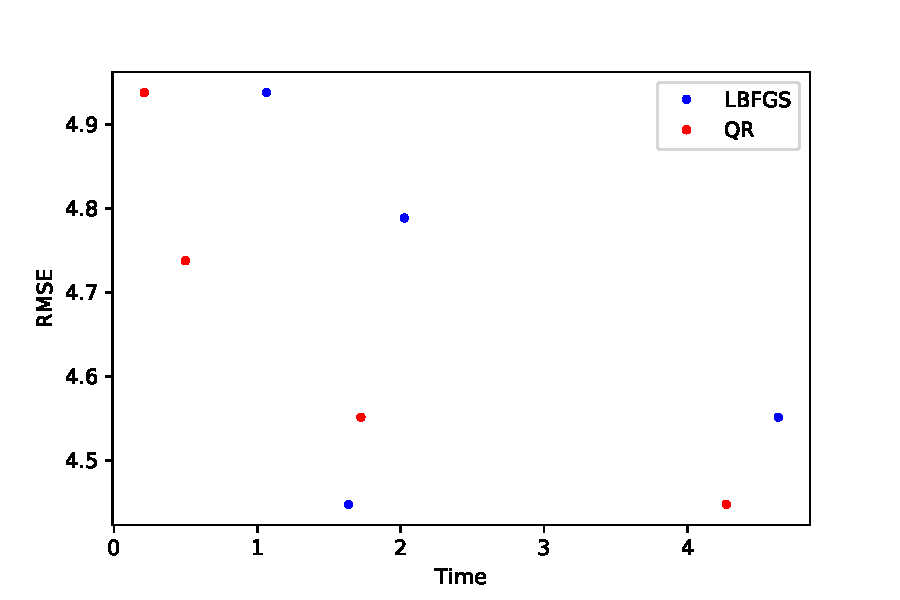
\includegraphics[scale=0.7]{rmse-time.pdf}
	\caption{Figure 1: RMSE vs. Time for LBFGS and QR}
\end{figure}
	\item Non-linear transformations help reduce the prediction error presumably because the underlying data has non-linear relationships in feature-space. Further, non-linear transformations allow us to increase the dimensionality of feature-space; therefore, we are not only able to capture more intricate non-linear relationships but also able to project our data onto a higher-dimensional space.
	\item QR is faster. This is perhaps because of implementation. We have written explicit loops into LBFGS, while for QR we have used optimized numpy matrices. Further LBFGS is iterative by design, and is making more complicated calculations.
\end{itemize}

\end{document}
